\documentclass[12pt,oneside]{fithesis2}
\usepackage[slovak]{babel}       % Multilingual support
\usepackage[utf8]{inputenc}       % UTF-8 encoding
\usepackage[T1]{fontenc}          % T1 font encoding
\usepackage[                      % A sans serif font that blends well with Palatino
  scaled=0.86
]{berasans}
\usepackage[                      % A tt font if you do not like LM's tt
  scaled=1.03
]{inconsolata}
\usepackage[                      % Clickable links
  plainpages = false,               % We have multiple page numberings
  pdfpagelabels                     % Generate pdf page labels
]{hyperref}
\usepackage{blindtext}            % Lorem ipsum generator
\usepackage{amsmath}

\usepackage{listings}
\lstset{language=C++}
\usepackage{verbatimbox}
\usepackage{graphicx}
\parskip 1ex
\parindent 0in

\thesislang{sk}                   % The language of the thesis
\thesistitle{Vyhľadávanie najbližších vektorov s využitím knižnice FLANN}       % The title of the thesis
\thesissubtitle{Bakalárska práca}  % The type of the thesis
\thesisstudent{Tomáš Durčák}          % Your name
\thesiswoman{false}                % Your gender
\thesisfaculty{fi}                % Your faculty
\thesisyear{Jar \the\year}     % The academic term of your thesis defense
\thesisadvisor{RNDr. David Novák, Ph.D.}   % Your advisor

\begin{document}
  \FrontMatter                    % The front matter
    \ThesisTitlePage                % The title page
    \begin{ThesisDeclaration}       % The declaration
      \DeclarationText
      \AdvisorName
    \end{ThesisDeclaration}
    \begin{ThesisThanks}            % The acknowledgements (optional)
      I would like to thank my supervisor\,\dots
    \end{ThesisThanks}
    \begin{ThesisAbstract}          % The abstract
      The aim of the bachelor work is to provide\,\dots
    \end{ThesisAbstract}
    \begin{ThesisKeyWords}          % The keywords
      keyword1, keyword2\,\dots
    \end{ThesisKeyWords}
    \tableofcontents                % The table of contents
%   \listoftables                   % The list of tables (optional)
%   \listoffigures                  % The list of figures (optional)
  
  \MainMatter                     % The main matter
    \chapter{Úvod}          % Chapters
    
    \chapter{Základné pojmy}
    
    	\section{Vektorový priestor}
    Vektorový priestor $ \Omega = D_1D_2. . .D_n $ má dimenziu $n$. Objekt (resp. vektor alebo bod)  $\mathcal{O} = [a_1, a_2, . . . , a_n] $ patriaci do vektorového priestoru je jednoznačne určeny svojimi súradnicami $ a_i \in D_i, 1 \le i \le n, $ ktorých je práve $n$. Každá jednotlivá dimenzia má svoju doménu $D_i$ - množinu hodnôt (resp. vlastností), ktoré môže prislušná vektorová súradnica nadobúdať. \cite{stromy}
    	
    Vektorový priestor $\Omega$, definujeme nad určitým poľom $\mathbf{P} $, s význačným prvkom $\mathbf{0}$ a dvomi binárnymi operáciami, sčítaním $+ : \Omega \times \Omega \rightarrow \Omega $  a násobením $. : \mathbf{P}  \times \Omega \rightarrow \Omega$, takými že platí: 
     
\begin{equation*}
\forall u,v,w \in \Omega : (u + v)+w = u+(v+w) 
\end{equation*}
\begin{equation*}
\exists\mathbf{0} \in \Omega : u+\mathbf{0} = \mathbf{0}+u = u
\end{equation*}
\begin{equation*}
\forall u \in \Omega \; \exists \; u \in \Omega : u+(-u)  = \mathbf{0}
\end{equation*}
\begin{equation*}
\forall a,b \in \mathbf{P} \; \exists \; u \in \Omega : (a.b).u = a.(b.u) 
\end{equation*}
\begin{equation*}
\forall u \in \Omega : 1.u=u  \textrm{ kde } 1 \in \mathbf{P}  \textrm{ je jednotkový prvok z } \mathbf{P} 
\end{equation*}
\begin{equation*}
\forall a,b \in \mathbf{P} \; \exists \;u \in \Omega : (a+b).u = a.u + b.u 
\end{equation*}
\begin{equation*}
\forall a \in \mathbf{P} \; \exists \;u,v \in \Omega : a.(u+v) = a.u + a.v 
\end{equation*} \\
\textbf{Poznámka:} Vektorový podpriestor je tiež vektorový priestor.

\begin{figure}
  \centering
  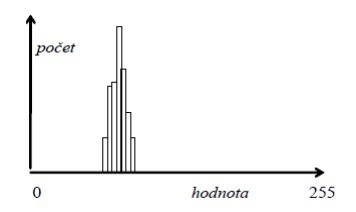
\includegraphics[width=6cm]{obr/gis_histogram_obrazu.png}
  \caption{Histogram farieb so siedmimi farebnými odtieňmi.}
  \label{fig:triangle}
\end{figure}  

\textbf{Príklad:}
Obrázok (resp. jeho histogram farieb) može byť vektorom vo vektorovom priestore a mať súradnice podľa počtu pixelov z každého farebného odtieňu.
Potom vektor z histogramu farieb je:
\begin{equation}
\{(\alpha_1,\beta_1),...(\alpha_M,\beta_M)\}
\end{equation}
kde $M$ je počet farebných odtieňov. \\
Iným príkladom môže byť dokument reprezentovaný ako
vektor v $m$-rozmernom priestore príznakov, ktoré zodpovedajú jednotlivým slovám – tzv.termom. Množina $n$ dokumentov je reprezentovaná ako matica $n\times m$. Neplnovýznamové slová (pomocne slovesá, spojky...) sa zvyčajne odstránia. \cite{vectorspace}


    \section{Metrický priestor}
    
    Metrický priestor je množina, na ktorej je definovaná vzdialenosť pre všetky prvky z množiny. Táto vzdialenosť sa nazýva metrika. Metriku môžme definovať ako funkciu, ktorá určuje vzdialenosť medzi dvomi objektami. \\ \\
    \textbf{Definícia:} Nech $X\neq 0$ je množina. Definujme zobrazenie \\ $d: X \times X \rightarrow R $, ktoré spĺňa nasledujúce vlastnosti:
    \begin{align*}
    \textrm{ Pre všetky } x,y,z \in X \qquad d(x,x) &= 0 \\
    d(x,y) &\textgreater 0 \qquad x\neq y \\
    d(x,y) &= d(y,x) \\
    d(x,z) + d(z,y) &\geq d(x,y)
    \end{align*}
    
    Množinu \textbf{$X$} nazývame \textbf{základnou množinou}, zobrazenie $d$ \textbf{metrikou} a usporiadanu dvojicu $(X,d)$ \textbf{metrickým priestorom}.
    V tej istej množine možme definovať rôzne metriky. Metrika $d$ musí byť vždy nezáporná. \cite{Yianilos:1993:DSA:313559.313789} \\ \\
    \textbf{Príklad:} 
    Vzdialenosť dvoch bodov na priamke v $ \mathbf{R} \quad d=|x-y| $ alebo v rovine v
     $\mathbf{R^2} \quad d = \sqrt{(x_1-y_1)^2+(x_2-y_2)^2}$.
    
	\section{Vzdialenostné funkcie}
	Vzdialenostné funcie predstavuju hlavný spôsob určenia blízkosti alebo podobnosti dvoch objektov v určitej doméne. Táto vzdialenosť može byť definovaná rôzne. Najčastejšie v zavislosti od použitého datového typu alebo účelu aplikácie.
	Vzdialenostné funkcie rozdeľujeme na dva zakladne typy podľa charakteru ich návratovej hodnoty:
	\begin{itemize}
	\item \textbf{diskrétne --} vracajú len vopred určenú množinu hodnôt malého rozsahu, napr. 	     len hodnotu $1$ alebo $-1$
	\item \textbf{spojité --} rozsah vrátenej množiny hodnôt je veľmi veľký alebo aj nekonečno, 		napr. hodnoty z intervalu $[0,1]$
	\end{itemize}
	Ďalej si popíšeme najčastejšie používané vzdialenostné funkcie. Jednu z nich budeme používať aj v testovaní a porovnávaní testovaných knižníc. \cite{Zezula2, Chavez:2001}
\subsection{Minkowského vzdialenosť}
Minkowského vzdialenosť je generalizovaná metrika, ktorá zahŕňa tzv. $L_p$ metriky v zovšebecnenej forme. Minkowskí ju definoval takto: 
\begin{equation*}
L_p((x_1,...,x_n),(y_1,...,y_n))=\sqrt[p]{\left(\sum\limits_{i=1}^n \mid x_i-y_i \mid^p \right)}
\end{equation*}
Rovnica udáva vzdialenosť medzi dvomi objektami v $n$-dimenzionalnom priestore pre $p\geq 1$ (ak by bolo $p \textless 1$ nešlo by o metriku). \cite{Zezula2} \\
	\begin{figure}
  		\centering
  		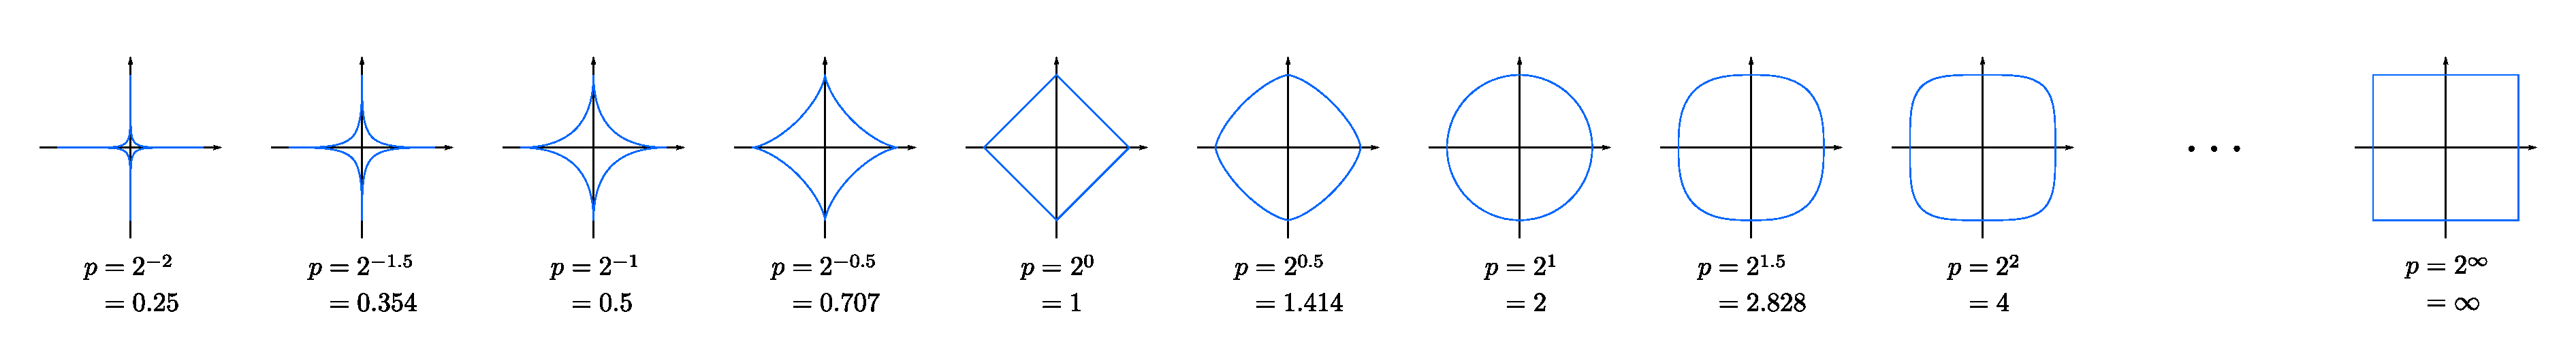
\includegraphics[width=14cm]{obr/lp.eps}
  		\caption{Znázornenie $L_p$- metrik v $R^2$ podľa parametra p}
  		%\label{fig:triangle}
	\end{figure}  

Medzi najznámejšie a napoužívanejšie metriky patria:
\begin{itemize}
\item $L_1$ -- Manhattanská metrika vyjadruje najkratšiu vzdialenosť, ktoru musíme prejsť aby sme sa v meste dostali z jedneho bodu do druhého. Je pomenovaná podľa pravouhélo systému ulíc v meste New York.
\item $L_2$ -- Eklidovská metrika vyjadruje najkračšiu vzdušnú vzdialenosť medzi dvomi objektmi. $L_2$ je použitá aj pri testoch.
\item $L_\infty $ -- Čebyševova metrika, nazýva sa tiež maximálna alebo šachovnicová vzdialenosť, pretože na šachovnici, je to minimalny počet ťahov potrebných na prejdenie kráľom z jedného štvorca na iný.
\end{itemize}
   \section{Vyhľadávanie v metrických a vektorových priestoroch}
   Základnou charakteristikou vyhľadávania vo vektorových a metrických priestoroch je neurčitosť. Týka sa to hlavne problému \textbf{Najdenia najbližšieho suseda} (ang. Nearest neighbor search) \cite{nns2009}. Tento problém obecne definujeme takto: \\
   Je daná množina bodov $P=\{p_1,...,p_n\}$ v priestore $X$ a dotazované body $q \in M$, nájdite najbližšie body z $P$ ku $q$.\\
   Pod pojmom \textbf{najbližši sused} rozumieme objekt alebo bod podobný dotazovanému bodu. Nepožadujeme aby boli vysledky vyhľadávania vždy na 100\% presné, ale aby výpočet skončil v čo najkratšom čase.
   Pred vyhľadávaním sa musíme rozhodnúť, ako chceme určovať blízkosť objektov, akú metriku použijeme. V našich testoch bola použitá $L_2$ metrika, čiže klasická Euklidovská metrika, ktorá je vhodná pre husto vzorkované dáta. Ďalej sa musíme rozhodnúť, koľko najbližšich susedov budeme hľadať. Existujú 3 základné druhy dotazov:
   \begin{itemize}
   \item \textbf{Dotaz na najbližšieho suseda}- hľadáme najližší najpodobnejší objekt k dotazu, výsledkom je 1 objekt ku každému dotazu.
   
   \textbf{Definícia:}
   \begin{equation*}
   NN(q)=\{x \in X, \forall y \in X| d(q,x)\leq d(q,y) \}
   \end{equation*}
Výsledkom je bod $x$, ktorého vzdialenosť od dotazu $q$ je najmenšia spomedzi všetkých bodov z množiny $X$.
   \item \textbf{Dotaz na k-najbližších susedov}- niekedy nám nemusí stačiť len 1 najbližší objekt, preto hľadáme $k$ susedov, ktoré sú mu podobné.
   
   \textbf{Definícia:}
   \begin{equation*}
   kNN(q)=\{A|A \subseteq X,|A|=k,\forall x \in A,\forall y \in X - A,d(q,x)\leq d(q,y)\}
   \end{equation*}    
   \item \textbf{Rozsahový dotaz}- použijeme, keď chceme nájsť všetkych najbližších susedov, ktorý su od dotazovaného bodu $q$ vzdialený maximálne zvolenú hodnotu $r$ (polomer vyhľadávania).
   
   \textbf{Definícia:} %R(q,r)=\{ x \in X|d(q,x)\leq r \}
   \begin{equation*} 
  rNN(q,X,r)=\{ x \in X|d(q,x)\leq r \}
   \end{equation*}  
   \end{itemize}
   
	\begin{figure}
  		\centering
  		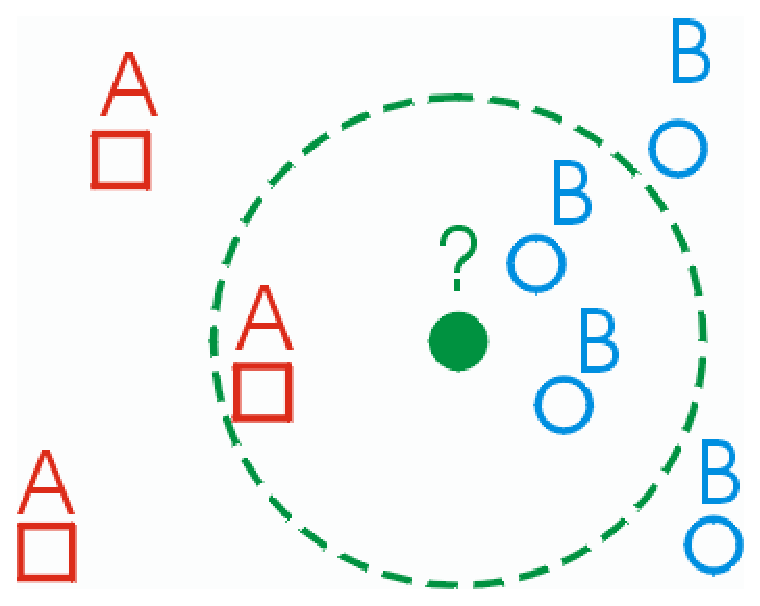
\includegraphics[width=6.5cm]{obr/Image25.eps}
  		\caption{Znázornenie $kNN$ a $rNN$ v $L_2$-metrike}
  		%\label{fig:triangle}
	\end{figure}  

\section{Indexové štruktúry}

Pri vyhľadávaní v metrických alebo vektorových prietoroch je vhodné dáta rozdeliť do menších podmnožin a niektoré data pri prezeraní vynechať, čím sa môže odpoveď na dotaz značne urýchliť. Na roztriedenie dát použivame špeciálne indexové štruktúry. Dve z nich si v podkapitolách popíšeme.
\subsection{KD-stromy}
KD = k-dimenzionálny strom \cite{Kibriya2007} je binárny strom slúžiaci na reprezentáciu priestorových dát vyšších dimenzií vo vektorovom priestore. Dáta sú v strome rozdeľované podľa viacdimenzionálnych kľúčov, ktorými su zvyčajne súradnice bodov alebo vektorov. \\ \\
\textbf{Vytvorenie KD-stromu}\\
\textbf{Vstup:} Množina objektov v k-dimenzionálnom priestore. \\
\textbf{Problem:} Vytvoriť strom, ktorý rozdeľuje priestor polrovinami, tzn. každý objekt je vo svojom vlastnom kvádri. Viď Obr. 2.4.\\
\begin{figure}
  		\centering
  		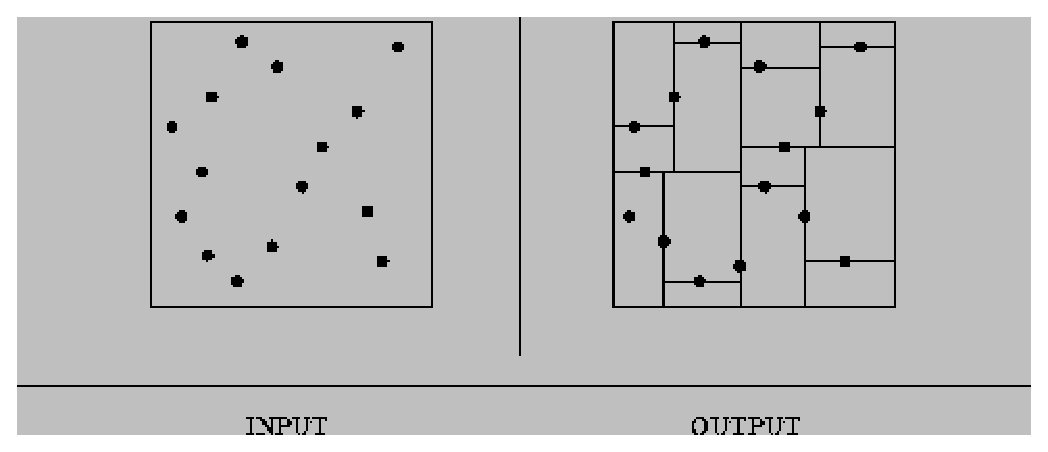
\includegraphics[width=13cm]{obr/kdtree.eps}
  		\caption{Znázornenie $kNN$ a $rNN$ v $L_2$-metrike}
  		%\label{fig:triangle}
\end{figure}
\textbf{Samotná konštrukcia stromu:} \\ 
-- v každej úrovni stromu vyberáme postupne jeden z koordinátov $ \{ x_1,x_2,...,x_k \} $ ako základ rozdeľovania ostaných objektov \\
-- napríklad v koreni stromu sa rozhodujeme podľa $x_1$ a ako v binárnom vyhľadávacom strome, všetky objekty s hodnotou koordinátu $x_1$ menšou ako hodnota koreňového uzlu budú v ľavom podstrome a s väčšou alebo rovnou hodnotou budú v pravom podstrom \\
-- v ďalšej podúrovniach stromu triedime objekty postupne podľa ďalších koordináttov, keď už bude mať strom hĺbku $k$, začíname porovnavať opäť od začiatku podľa $x_1,...$ \\
-- ak by sme vkladali objekty do stromu v nahodnom poradí, strom by bol nevyváženy, preto sa vkladané objekty vyberajú podľa priemernej hodnoty všetkých hodnôt na danom koordináte alebo podľa mediánu \\
-- po log(n) krokoch sa rozklad zastaví, každý objekt má svoje miesto\\ \\
\textbf{Vkladanie objektu do stromu:}\\
\textbf{Príklad:} Do stromu na Obr. 2.5 vložíme objekt s kľúčom (11,8)\\
-- v koreni sa podľa koordinátu $x$ porovná s uzlom (7,2), kedže 11>7 ide doprava \\
-- v ďalšej urovní sa porovná podľa $y$ s uzlom (9,6), kedže 8>6 ide doprava, tento uzol je prázdny, preto sa na toto miesto uloži objekt (11,8) \\ \\
\begin{figure}
  		\centering
  		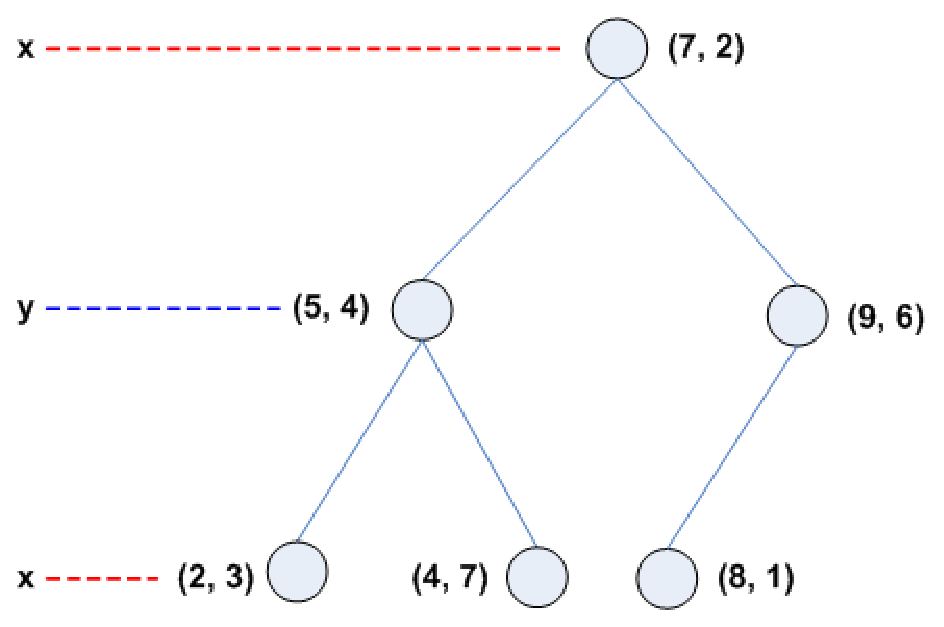
\includegraphics[width=7cm]{obr/Kd_tree.eps}
  		\caption{Vkladanie objektu do KD-stromu}
  		%\label{fig:triangle}
\end{figure}
\textbf{Vyhľadávanie v KD-strome} \\
KD-strom umožňuje vyhľadávať najbližšie body. Na Obr. 2.4 je znázornené ako strom rozdelí vektorový priestor na menšie obdĺžniky -- polroviny. Nájdenie najbližšieho objektu teda znamená najdenie oblasti, v ktorej je dotaz $q$ a prehľadanie okolitých oblastí, kde by sa ešte mohol nachádzať ešte bližší bod.
\\
\textbf{Algoritmus:} \\--nájde sa bunka $c$ obsahujúca objekt $q$ \\
--$q$ je ohraničená nejakým objektom $p$ (to ale nemusí byť najližší objekt)\\
--nájdeme všetky najbližšie bunky $c'$ vo vzdialenosti $d(p,q)$ \\
--otestujeme či $c'$ neobsahuje bližší objekt \\
\\
\textbf{Použitie:}\\
KD-stromy sa používajú hlavne na indexovanie objektov s nižšou dimenziou. Pri vyšších dimenziách sa začne prejavovať tzv. \textit{prekliatie dimenzionality}, ktoré spôsobuje neefektívnosť pri vyhľadávaní.

  
\subsection{M-stromy}
   Pre indexovanie objektov v metrických priestoroch sa často využíva datová štruktúra M-strom \cite{stromy}. Štruktúru stromu tvorí opäť n-arny strom ako u KD-stromu. Rozdiel spočíva v obsahu uzlov a listov stromu. Samotné objekty sú uložené len v listových uzloch stromu. Nelistové ulzy obsahujú tzv. \textbf{smerovacie objekty}. \\\\
Každý smerovací objekt v uzle obsahuje:
\begin{itemize}
\item Samotný objekt $O_r$, ktorý može byť \textit{virtuálny} -- vypočítaný pre účely M-stromu alebo \textit{skutočný} -- uloženy v niektorom liste $T(O_r)$
\item Odkaz $ptr(T(O_r))$ n svoj podstrom $T(O_r)$
\item Polomer $r(O_r)$
\item Vzdialenosť $d(O_r,P(O_r))$  od svojho rodičovského smerovacieho objektu $P(O_r)$
\end{itemize}
Listove uzly vypadajú podobne, ale miesto odkazu na svoj podstrom a polomeru obsahujú $oid(O_j)$ -- identifikátor celého objektu.\\

Princíp hierarchie M-stromu spočíva rovnako ako u KD-stromu v rozdelení priestoru na menšie regióny, ktoré ale nemusia byť nutne disjunktné ako je to u KD-stromu. K rozdeleniu slúžia smerovacie objekty, pričom všetky objekty v listových uzloch, ktoré obsahuje podstrom $T(O_r)$ smerovacieho objektu $O_r$, sú vo vzdialenosti maximálne $r(O_r)$ od $O_r$. Teda:
\begin{equation*}
\forall O_i \in T(O_r) \qquad   d(O_r,O_i) \leq r(O_r)
\end{equation*}
\begin{figure}
  		\centering
  		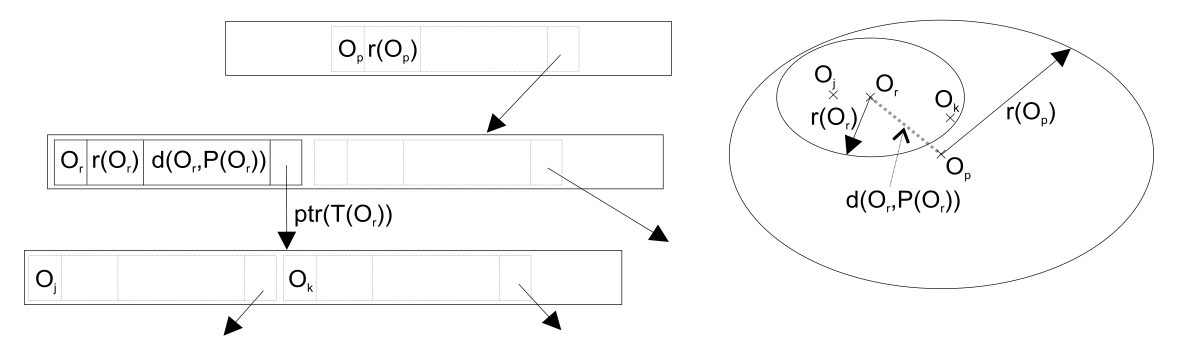
\includegraphics[width=13cm]{obr/m-tree.png}
  		\caption{Uzly M-stromu obsahujúce objekty (vľavo) a regióny smerovacích objektov znazornené v metrickom priestore (vpravo)} Zdroj: \cite{stromy} 
  		%\label{fig:triangle}
  		\label{m-strom}
\end{figure}
Na obrázku \ref{m-strom} je znázornená štruktúra stromu a vzťahy medzi smerovacími objektami.\\
\\
\textbf{Vytvorenie M-stromu:}\\
Rovnaká množina objektov može byť v M-strome indexovaná mnohými rôznymi spôsobmi, pričom neporušíme ani jeden z axiomov metriky alebo vlastnosti M-stromov. Avšak každý z tychto zpôsobov memusí byť práve ideálny z hľadiska efektivity operácií vykonávaných nad M-stromom. Obecne hľadáme také spôsoby konštrukcie stromov, aby zložitost dotazovania bola minimálna. Efektívnosť vyhľadávania v značnej miere ovplyvňuje výber smerovacích objektov tzv. \textit{pivotov}, ktoré potrebujeme na rozdelenie metrického priestoru pri vytváraní stromu. Dôležitý je vyber pivotov, ktorí sú vo vhodnej vzdialenosti od osnatných objektov. Dobrí pivoti by mali byť navzájom ďaleko od seba a taktiež by sa mali nachádzať ďaleko od ostatných objektov v metrickom priestore. \\
\\
\textbf{Vyhľadávanie v M-strome:}\\
V M-stromoch môžme vyhľadávať \textit{k-najbližších susedov} ako aj pomocou \textit{rozsahového dotazu}. 

Pri vyhľadávaní k-najbližších susedov je dôležitá prioritná rada, z ktorej postupne vyberáme objekty na vyhľadávanie v strome $T(O_r)$. Každý objekt v rade má tvar:\\ $(prt(T(O_r)), d_{min}(T(O_r)))$. Prvý člen je už známy ukazateľ na podstrom, druhý člen je spodná hranica medzi dotazovaným objektom $Q$ a každým objektom $O_j$ z $T(O_r)$.
\\ \\
\textbf{Použitie:} \\
M-stromy požívame, keď dáta nie je možné indexovať vo vektorovom priestore, alebo keď sú vektory dát príliš dlhé (dimenzia \textgreater \,20). Metrický priestor umožňuje definovať špeciálne metriky a tým rôzne interpretovať vzdialenosť (resp. podobnosť) objektov na základe ich vlastností.

	\chapter{Knižnica FLANN}
	FLANN\footnote{Z anglického: Fast Library for Approximate Nearest Neighbors} je knižnica poskytujúca rýchly programátorsky nástroj, ktorý slúži na \textit{vyhľadávanie najbližších susedov}. Pre tento účel obsahuje kolekciu nástrojov (algoritmov) a tiež systém automatického výberu najlepšieho algoritmu a optimálnych parametrov použitých pri vyľadávani najbližších susedov. Aby bolo vyhľadávanie čo najrýchlejšie, je knižnica FLANN napísaná v programovacom jazyku C++ a je možné ju použiť aj pri programovaní v jazykoch C, Matlab, Python a Ruby. Knižnica je voľne šíriteľná pod licenciou BSD\footnote{BSD licencia sa používa pre voľne šíriťeľný softvér, je pomenovaná podľa Berkeley Software Distribution, UNIXový operačný systém}.\cite{flann_pami_2014}
	
V ďalších podkapitolách si popíšeme algoritmy \textit{priority search
k-means tree}\footnote{Algoritmus pre prioritné K-means stromy} a \textit{multiple randomized k-d trees}\footnote{Algoritmus náhodných KD-stromov}, ktoré sú obsiahnuté v knižnci FLANN a javia sa najrýchlejšie z pomedzi existujúcich algoritmov na vyhľadávanie najbližších susedov.
	\section{Algoritmus náhodných KD-stromov}
Klasické algoritmy výužívajúce KD-stromy sú vhodné na vyhľadávanie najbližších susedov v nízko-dimenzionálnych dátach, avšak pre vyššie dimenzie vykazujú značný pokles výkonu. Tento problém viedol k vývoju nového a vylepšeného algoritmu využívajúceho KD-stromy. \cite{flann_pami_2014}	
	
	Algoritmus je založený na stavaní mnohopočetných nahodných KD-stromov, ktoré sú prehľadávané paralelne. Originálne KD-stromy pri výtvaraní delia dáta na polovicu v každej úrovni stromu vždy postupne podľa dimenzií zaradom. Na porovnanie nahodne KD-stromy vyberajú deliacu dimenziu náhodne z prvých $D$ dimenzií, kde majú dáta najväčší rozptyl. Knižnica FLANN používa v implementácií algoritmu hodnotu $D$ = 5, ktorá sa pri testoch ukázala ako optimálna. Pri vyhľadávani sa používa prioritná rada skrz všetky randomizované KD-stromy. Objekty v tejto rade sú zoradené podľa zvyšujúcej sa vzdialenosti od deliacej hranice v každej úrovni, čo zvyšuje rychlosť vyhľadávania. Každý objekt, ktorý už bol porovnaný s dotazom v niektorom strome, je označený a v ďalších  stromoch sa už neporovnáva. Presnosť aproximácie vyhľadávania sa reguluje nastavením maximálneho počtu listových uzlov (skrz všetky stromy), ktoré sa pri vyhľadávaní skontrolujú. \cite{flann_pami_2014} 	
	
	\section{Algoritmus pre prioritné K-means stromy}
	Pri niektorých typoch dát, može byť efektívnejší algortmus K-means stromov, vzlášt ak je prioritou vysoká presnosť výsledkov. Algoritmus prioritných K-means stromov sa snaží lepšie využívať prirodzenú štruktúru vstupných dát. Na rozdiel od randomizovaných KD-stromov, delí a zoskupuje data do skupín za základe vzdialeností skrz všetky dimenzie, pričom KD-stromy využívajú na delenie v každej úrovni len jeden rozmer. \cite{flann_pami_2014}
	\subsection{Opis algoritmu}
	Pri tvorení K-means stromu sa dáta delia v každej úrovni do $K$ rôznych regiónov pomocou \textit{K-means zhlukovacieho algoritmu}. Rovnaká metóda sa rekurzívne aplikuje na každu novú skupinu dát. Delenie končí, keď počet objektov v každom regióne je menší ako hodnota $K$. Presnejší popis a štruktúra algoritmu \cite{flann_pami_2014}.
	\subsection{Výhľadávanie v strome}
	K-means strom sa prehľadáva postupne od koreňa k najbližšiemu listu. Vetvy, ktoré boli pri prechádzaní stromu preskočené sa ukladajú do prioritnej rady, zoradené podľa vzdialenosťi k dotazovanému objektu. Algoritmus potom ešte skontroluje podstromy uložené v tejto rade. Presnejší náhľad algoritmu je opäť v \cite{flann_pami_2014}.
	
	Počet regiónov $K$, na ktoré sa vstupné dáta delia pri vytváraní stromu určuje parameter algoritmu nazvaný \textit{počet vetiev stromu}. Výber optimálneho $K$ ovplyvňuje rýchlosť a správnosť vyhľadávania. Ďalším parametrom je $I_{max}$ a určuje maximálny počet iterácií, ktoré sa vykonajú pri delení stromu na regióny. Menší počet iterácié urýchli stavbu stromu, ale zníži presnosť vyhľadávania. Posledným parametrom je výber algoritmu, ktorý určí ako sa bude počítať rozhodovacia hranica pri delení objektov do regiónov. K dispozícií mame: \textit{náhodný výber}, \textit{Gonzalesov algoritmus} (výber objektov, ktoré su ďaleko od seba) alebo  \textit{KMeans++ algoritmus} \cite{K-means++}. \cite{flann_pami_2014}
	
	\section{Algoritmus The Hierarchical Clustering Tree\protect\footnote{Algoritmus pre Hierarchické zhlukovacie stromy}}
	Prechádzajúce dva algoritmy sú určené predovšetkým na vyhľadávanie najbližších susedov vo vektorových dátach. Niesu však vhodné na vyhľadávanie v binárnych dátach. Pre tento účel bol vyvinutý nový algoritmus, ktorý výužíva novú datovú štruktúru: \textit{hierarchické zhukovacie stromy}. \cite{Attach:binary_matching_crv2012}
	
	Vytváranie hierarchického zhlukovacieho stromu je podobné K-means stromu.   Zo vstupných dát sa nahodne vyberie $K$ \textit{zhlukovacích centier} a objekty sa rozdelia do $K$ zhlukov podľa toho, ku ktorému zhlukovaciemu centru sú najbližšie. Hodnota $K$ je vstupný parameter algoritmu. Delenie potom prebieha rekurzívne na všetkych nových zhlukoch, až kým nie je počet objektov v zhluku menši ako $K$. Vtedy sa vytvoria listové uzly stromu. \cite{Attach:binary_matching_crv2012}
	
	Na rozdiel od algoritmu pre prioritné K-means stromy, nevytvárame zo vstupných dát len jeden strom, ale celý les stromov, v ktorom sa vyhľadáva paralelne. Aby bolo vytváranie stromov rýchlejšie, je výhodné vyberať zhukovacie centrá náhodne, pričom nedochádza k výraznému poklesu presnosti. Vyhľadávanie je podobné algoritmu pre K-means stromy. \cite{Attach:binary_matching_crv2012}
	
	Pred vytváraním stromu možme nastaviť \textit{rozvetvenie stromu ($K$)}, \textit{počet stromov}, \textit{maximálny počet objektov v listových uzloch} a \textit{algoritmus pre výber prvých $K$ zhukovacích centier}. \cite{Attach:binary_matching_crv2012}
	
	\section{Automatický výber algoritmu}\label{sec:autotuning}
	Výber správneho algoritmu a optimálnych parametrov pri vyhľadávanie najbližších susedov nie je triviálny problém. Správný voľba závisí od niekoľkých faktorov ako napríklad: štruktúra vstupných dát a zvolená presnosť vyhľadávania. Každý z možných algoritmov má množinu nastaviteľných parametrov, ktoré v značnej miere ovplyvňujú výsledky vyhľadávania. Je to napríklad počet náhodných stromov pri použití KD-stromu alebo počet vetiev každého uzla pri hierarchickom K-means strome. \cite{muja_flann_2009} 
	
	Výber algoritmu je optimalizačný problém, ktorým sa snažíme nájsť najlepšie riešenie. Cenú výpočtu počítame ako kombináciu času potrebného na vyhľadávanie dotazov, času za ktorý sa vytvorí vyhľadávací index (strom) a pamäťovej záťaže. Každy z týchto faktorov má inú váhu v závislosti na aplikácií a použití. Ak vytvárame vyhľadávací index len raz, ale vyhľadávanie prebieha mnohokrát, je dôležitejší čas vyhľadávania ako čas potrebný na vytvorenie indexu. Niekedy vyhľadávame v indexe len raz, napríklad pri on-line aplikáciach, vtedy potrebujeme aby sa index vytvoril čo najrýchlejšie. Môžu nastať aj situácie, kedy potrebuje čo najmenšie pamäťová zaťaženie.Váha pamäťového zaťaženie je $w_m$ a váha času vytvorenie indexu je $w_b$. Celkovú cenu počitame pomocou:
	\begin{equation}
	\mathrm{cost} = \dfrac{s + w_bb}{(s + w_bb)}_{opt} + w_mm
	\label{cena}
	\end{equation}
kde $s$ je čas vyhľadávania a $b$ je čas potrebný na vytvorenie vyhľadávacieho indexu. Parameter $m = m_t/m_d$ reprezentuje pomer pamäte použitej na uloženie indexu ($m_t$) a uloženia dát ($m_d$). Parameter $w_b$ reguluje čas potrebný na vytvorenie indexu vzhľadom ku času vyhľadávania. Ak nastavíme $w_b = 0$, znamená to, že chceme čo najrýchlejšie vyhľadávať a nezaujíma nás rýchlosť vytvorenia indexu. Nastavením $w_b = 1$, priradíme času vyhľadávania a vytvorenia indexu rovnaku doležitosť. Podobne $w_m$ nastavuje prioritu medzi časom (čas vyhľadávania vytvorenia indexu) a pamäťou, ktorú využiva vyhľadávací index. Hodnota $w_m \textless 1$ kladie väčšiu váhu na čas nehľadiac na pamäť a hodnota $w_m \textgreater 1$  kladie prioritu na množstvo využitej pamäte. Nastavením $w_m = 1$ priradíme rovnakú prioritu času aj využitiu pamäte. \cite{muja_flann_2009} 

Výber najlepšieho algoritmu a optimálnych parametrov sa vykonáva v dvoch ktorokoch: V prvom kroku vyberáme algoritmus s najlepšimi výsledkami podľa rovnice \ref{cena}. Pri testovaní sa využívaju hodnoty z množiny \{1,4,8,16,32\} ako počet náhodných KD-stromov, \{1,5,10,15\} ako počet iterácií a \{16,32,64,128,256\} ako počet vetiev v K-means strome. V druhom kroku sa využíva Nelder-Mead downhill simplex metóda \cite{NelderMead65}, pomocou ktorej sa určia optimálne parametre pre algoritmus vybraný v prvom kroku. Optimalizácia može byť počítaná na celých vstupných dátach, alebo len na časti. Typicky stačí $5-10\,\%$ a výsedky sa stále veľmi blížia optimálnym hodnotám (ak sú dáta podobnej štruktúry). \cite{muja_flann_2009} 

	\section{Použitie knižnice FLANN v C++}
	Jadro knižnice FLANN je naprogramované v programovacom jazyku C++, preto je na jej samotnú kompiláciu potrebný C++ prekladač. Knižnicu je možne použiť Linuxovými distribúciami ale aj Windowsom a OS X. Pre viac-jadrovú podporu je nutné mať nainštalovanú knižnicu OpenMP. Predkompilovanú knižnicu FLANN je  možné použiť aj pomocou knižnice PCL (Point Cloud Library)\footnote{http://www.pointclouds.org}, do ktorej je implementovaná jedna zo starších verzií. V ďalších častiach si popíšeme niektoré základné triedy a funkcie knižnice. \cite{manual}
	
	\subsection{Trieda flann::Index}  
	Táto trieda tvorí základ knižnice. Je abstraktnou triedou pre všetky typy indexov a je šablonovaná na rôzne druhy vzdialenostných funkcií. \cite{manual}\\
\textbf{Konštruktor:}

{\scriptsize	
\begin{lstlisting}[frame=single]  
Index(const IndexParams& params, Distance distance = Distance() );

Index(const Matrix<ElementType>& points, const IndexParams& params,
       Distance distance = Distance() );
\end{lstlisting}}
Trieda \textbf{Matrix<ElementType>} obsahuje uložené objekty, z ktorých sa má vytvoriť vyhľadávací index. Objekty sú uložené v poradí za sebou. \cite{manual}

\textbf{IndexParams} je štruktúra, ktorá obsahuje parametre indexu. Typ indexu, ktorý sa vytvorí zavysí na tomto parametri. IndexParams može mať rôzne typy:
\begin{itemize}

\item \textbf{LinearIndexParams} Index s týmto typom vyhľadáva najbližšie objekty pomocou lineárneho vyhľadávania. \cite{manual}

\item \textbf{KDTreeIndexParams} Index s týmto typom vytvorí randomizované KD-stromy, ktoré sa prehľadávajú pararelne. V štruktúte je možné nastaviť počet stromov (\texttt{trees}), ktoré sa majú vytvoriť. \cite{manual}
{\scriptsize
\begin{lstlisting}
struct KDTreeIndexParams : public IndexParams
{
	KDTreeIndexParams( int trees = 4 );
};
\end{lstlisting}}
\item \textbf{KMeansIndexParams} Index s týmto typom vytvorí hierarchický k-means strom.
{\scriptsize
\begin{lstlisting}
struct KMeansIndexParams : public IndexParams
{
	KMeansIndexParams( int branching = 32,
		int iterations = 11,
		flann_centers_init_t centers_init = FLANN_CENTERS_RANDOM,
		float cb_index = 0.2 );
};
\end{lstlisting}}
V štruktúre môžme nastaviť rozvetvenie stromu (\texttt{branching}), počet iterácií (\texttt{iterations}) alebo algoritmus na výber deliacej hranice (\texttt{centers\_init}). Hodnota \texttt{cb\_index} určuje, ktore objekty sa pri prechádzaní stromu porovnávajú ako prvé. Ak je \texttt{cb\_index} = 0, uprednostňujú sa objekty bližšie k deliacej hranici. \cite{manual}

\item \textbf{CompositeIndexParams} Index s týmto typom je kombináciou randomizovaných KD-stromov a hierarchického K-means stromu. \cite{manual}
{\scriptsize
\begin{lstlisting}
struct CompositeIndexParams : public IndexParams {
	CompositeIndexParams( int trees = 4,
		int branching = 32,
		int iterations = 11,
		flann_centers_init_t centers_init = FLANN_CENTERS_RANDOM,
		float cb_index = 0.2 );
};
\end{lstlisting}} 

\item \textbf{KDTreeSingleIndexParams} Index s týmto typom vytvorí jeden KD-strom, ktorý sa hodí a je optimalizovaný na vyhľadávanie v nízkodimenzionálnych dátach (napríklad 2D a 3D priestor).
{\scriptsize
\begin{lstlisting}
struct KDTreeSingleIndexParams : public IndexParams
{
	KDTreeSingleIndexParams( int leaf_max_size = 10 );
};
\end{lstlisting}}
\texttt{leaf\_max\_size} nastavuje maximálny počet objektov v listových uzloch. \cite{manual}

\item \textbf{KDTreeCuda3dIndexParams} Index s týmto typom vytvorí jeden KD-strom. Vytvorenie a vyhľadávanie v strome prebieha na CUDA kompatibilných grafických kartách. Tento typ indexu sa hodí na vyľadávanie veľkého počtu dotazov. \cite{manual}

\item \textbf{HierarchicalClusteringIndexParams} Index s týmto typom použíje na vyhľadávanie hierarchické zhlukovacie stromy. \cite{manual}
{\scriptsize
\begin{lstlisting}
struct HierarchicalClusteringIndexParams : public IndexParams
{
	HierarchicalClusteringIndexParams(int branching = 32,
		flann_centers_init_t centers_init = FLANN_CENTERS_RANDOM,
		int trees = 4, 
		int leaf_max_size = 100)
};
\end{lstlisting}}
\item \textbf{AutotunedIndexParams} Tento typ indexu je určený pre automatický výber najlepšej vyhľadávacej štruktúry a jej optimálnych parametrov. \cite{manual}
{\scriptsize
\begin{lstlisting}
struct AutotunedIndexParams : public IndexParams
{
	AutotunedIndexParams( float target_precision = 0.9,
		float build_weight = 0.01,
		float memory_weight = 0,
		float sample_fraction = 0.1 );
};
\end{lstlisting}}
Parameter \texttt{target\_precision} určuje požadovanú presnosť vyhľadávania, parametre \texttt{build\_weight} a \texttt{memory\_weight} su podrobnejšie vysvetlené v podkapitole \ref{sec:autotuning}, kde predstavujú parametre $w_b$ a $w_m$. Parameter \texttt{sample\_fraction} može byť hodnota medzi 0 a 1, a určuje koľko percent objektov, v ktorých sa má vyhľadávať, sa využije na výpočet optimálneho algoritmu a parametrov. \cite{manual}

\item \textbf{SavedIndexParams} Umožňuje načítať predtým vytvorený a uložený index. \cite{manual}
{\scriptsize
\begin{lstlisting}
struct SavedIndexParams : public IndexParams
{
	std::string filename;
};
\end{lstlisting}}
\end{itemize}
	\subsection{Metodý triedy flann::Index} 
\begin{itemize}
	\item \textbf{flann::Index::buildIndex} Metóda vytvorí vyhľadávací index. K dispozícií sú dve preťažené varianty, jedna vytvorí index z dát poskytnutých v konštruktore Indexu, druhá varianta použije dáta z argumetu metódy. \cite{manual}
{\scriptsize
\begin{lstlisting}
void buildIndex();
void buildIndex(const Matrix<ElementType>& points);
\end{lstlisting}}

	\item \textbf{flann::Index::addPoints} Metóda umožňuje pridať objekty do indexu, potom ako už bol vytvorený. Hodota \texttt{rebuild\_threshold} umožňuje nastaviť, kedy sa má index prestavať, špeciálne pri veľkom počte pridávaných objektov. Prednastavená hodnota 2 znamená prestavanie indexu pri zdvojnásobení počtu objektov. \cite{manual}
{\scriptsize
\begin{lstlisting}
void addPoints(const Matrix<ElementType>& points, 
	float rebuild_threshold = 2);
\end{lstlisting}}	

	\item \textbf{flann::Index::removePoint} Metóda umožňuje odstrániť z indexu objekt s jedinečným identifikačným čislom \texttt{point\_id}. \cite{manual}
{\scriptsize
\begin{lstlisting}
void removePoint(size_t point_id);
\end{lstlisting}}
		
	\item \textbf{flann::Index::getPoint} Metóda vráti ukazateľ na objekt s identifikačným číslom \texttt{point\_id}. Index je neskôr možne opätovne použiť. \cite{manual}
{\scriptsize
\begin{lstlisting}
ElementType* getPoint(size_t point_id);
\end{lstlisting}}	

	\item \textbf{flann::Index::save} Metóda uloží vytvorený index do súboru \texttt{filename}. \cite{manual}
{\scriptsize
\begin{lstlisting}
void Index::save(std::string filename);
\end{lstlisting}}
	
	\item \textbf{flann::Index::knnSearch} Metóda na vyhľadávanie K-najbližších susedov pre množinu dotazovaných objektov, ktoré su uložene v objekte \texttt{queries} triedy \texttt{Matrix}. Argumenty \texttt{indices} a \texttt{dists} slúžia a uloženie výsledkov vyhľadávania. Argument \texttt{knn} určuje počet najbližších susedov, ktorý sa maju vyhľadať. 
{\scriptsize
\begin{lstlisting}
int Index::knnSearch(const Matrix<ElementType>& queries,
	Matrix<int>& indices,
	Matrix<DistanceType>& dists,
	size_t knn,
	const SearchParams& params);
\end{lstlisting}}
Argument \texttt{params} je štruktúra, ktorá nastavuje špecialne parametre použité počas vyhľadávania.
{\scriptsize
\begin{lstlisting}
struct SearchParams
{
	SearchParams(int checks = 32,
		float eps = 0,
		bool sorted = true);
	int checks;
	float eps;
	bool sorted;
	int max_neighbors;
	tri_type use_heap;
	int cores;
	bool matrices_in_gpu_ram;
};
\end{lstlisting}}
Hodnota \texttt{checks} určuje počet listových uzlov, ktoré sa maju skontrolovať a može byť nastavená na špecialne hotnoty:\\ \texttt{FLANN\_CHECKS\_UNLIMITED} (skontroluje všetky listové uzly),\\ \texttt{FLANN\_CHECKS\_AUTOTUNED} (použije vypočítanú hodnotu, ak bol index vytvorený automaticky). Môžme tiež nastaviť, či majú byť výsledky zoradené podľa vzdialeností (\texttt{sorted = true}) alebo počet jadier procesora, použitých pri vyhľadávaní (\texttt{cores}). \cite{manual}

	\item \textbf{flann::Index::radiusSearch} Metóda na rozsahové vyhľadávanie najbližších objektov do vzdialenosti polomeru \texttt{radius}. \cite{manual}
{\scriptsize
\begin{lstlisting}	
int Index::radiusSearch(const Matrix<ElementType>& queries,
	Matrix<int>& indices,
	Matrix<DistanceType>& dists,
	float radius,
	const SearchParams& params);
\end{lstlisting}}	
		
	\item \textbf{flann::hierarchicalClustering}
	
	\item \textbf{flann::KdTreeCuda3dIndex}
	
\end{itemize}		

    \chapter{Výsledky testov}

    \chapter{Záver}
    
\bibliographystyle{unsrt}
\bibliography{citacie}{}

    % Bibliography goes here
    % Index goes here (optional)
\end{document}
